\documentclass[a4 paper]{article}

\usepackage[inner=2.0cm,outer=2.0cm,top=2.5cm,bottom=2.5cm]{geometry}
\usepackage{setspace}
\usepackage[rgb]{xcolor}
\usepackage{verbatim}
\usepackage{subcaption}
\usepackage{amsgen,amsmath,amstext,amsbsy,amsopn,tikz,amssymb,tkz-linknodes}
\usepackage{fancyhdr}
\usepackage[colorlinks=true, urlcolor=blue,  linkcolor=blue, citecolor=blue]{hyperref}
\usepackage[colorinlistoftodos]{todonotes}
\usepackage{rotating}
\usepackage{graphicx}
\usepackage{minted}

\setlength{\parindent}{0pt}

\allowdisplaybreaks
\DeclareMathOperator*{\argmin}{\arg\min} 
\DeclareMathOperator*{\argmax}{\arg\max} 

\hypersetup{%
pdfauthor={Vineeth S},%
pdftitle={Homework},%
pdfkeywords={Tikz,latex,bootstrap,uncertaintes},%
pdfcreator={PDFLaTeX},%
pdfproducer={PDFLaTeX},%
}

\usepackage{booktabs}
\newcommand{\ra}[1]{\renewcommand{\arraystretch}{#1}}

\newtheorem{thm}{Theorem}[section]
\newtheorem{prop}[thm]{Proposition}
\newtheorem{lem}[thm]{Lemma}
\newtheorem{cor}[thm]{Corollary}
\newtheorem{defn}[thm]{Definition}
\newtheorem{rem}[thm]{Remark}
\numberwithin{equation}{section}

\newcommand{\homework}[6]{
   \pagestyle{myheadings}
   \thispagestyle{plain}
   \newpage
   \setcounter{page}{1}
   \noindent
   \begin{center}
   \framebox{
      \vbox{\vspace{2mm}
    \hbox to 6.28in { {\bf E1 244:~Detection and Estimation Theory\hfill {\small (#2)}} }
       \vspace{6mm}
       \hbox to 6.28in { {\Large \hfill #1  \hfill} }
       \vspace{6mm}
       \hbox to 6.28in { {\it Instructor: {\rm #3} \hfill Name: {\rm #5}, SR No.: {\rm #6}} }
       %\hbox to 6.28in { {\it TA: #4  \hfill #6}}
      \vspace{2mm}}
   }
   \end{center}
   \markboth{#5 -- #1}{#5 -- #1}
   \vspace*{4mm}
}

\newcommand{\problem}[2]{~\\\fbox{\textbf{PART #1}}\hfill \newline\newline}
\newcommand{\subproblem}[1]{~\newline\textbf{#1}}
\newcommand{\D}{\mathcal{D}}
\newcommand{\Hy}{\mathcal{H}}
\newcommand{\VS}{\textrm{VS}}
\newcommand{\solution}{~\newline\textbf{\textit{(Solution)}} }

\newcommand{\bbF}{\mathbb{F}}
\newcommand{\bbX}{\mathbb{X}}
\newcommand{\bI}{\mathbf{I}}
\newcommand{\bX}{\mathbf{X}}
\newcommand{\bY}{\mathbf{Y}}
\newcommand{\bepsilon}{\boldsymbol{\epsilon}}
\newcommand{\balpha}{\boldsymbol{\alpha}}
\newcommand{\bbeta}{\boldsymbol{\beta}}
\newcommand{\0}{\mathbf{0}}
\linespread{1.5}


\begin{document}

\setlength{\abovedisplayskip}{3pt}
\setlength{\belowdisplayskip}{3pt}

\homework{Assignment \#2}{Due: 22/05/20}{Sundeep Chepuri}{}{Vineeth S}{16543}

We are given $x(n)$ is a zero-mean real-valued wide-sense stationary (WSS) random process with autocorrelation sequence $ r(k)$. More specifically, the signal $x(n)$ is Autoregressive process of order 1 that is generated by the difference equation,
\begin{equation*}
x(n) = \alpha x(n - 1) + w(n)
\end{equation*}
where $w(n)$ is white noise with variance $\sigma_{w}^{2}$. We have access to the data set $\mathbf{x} = [x(0), x(1), ..., x(n -1)]^{T}$ or its noisy version. We want to estimate or interpolate $x(n_{0})$ where $n_{0}$ is the index of the sensor which is faulty.

\problem{A: Problem 1 LMMSE (Wiener) interpolator}{}{}
\solution Consider the class of LMMSE interpolators given,
\begin{align*}
	\hat{x}(n_{0}) &= \sum_{\substack{i = 0 \\ i \neq n_{0}}}^{N - 1} a_{i}x(i) \\
		&= \underline{a}^{T} \underline{x}
\end{align*}
where,
\[
\underline{a} = 
\begin{bmatrix}
	a_{0}	\\ a_{1}	\\ ..	\\ a_{n-1}	\\ a_{n+1}	\\ ..	\\	a(N-1)
\end{bmatrix}
\hspace{4em}
\underline{x} = 
\begin{bmatrix}
	x_{0}	\\ x_{1}	\\ ..	\\ x_{n-1}	\\ x_{n+1}	\\ ..	\\	x(N-1)
\end{bmatrix}
\]

We have the Bayesian Mean Squared Error (BMSE) as,
\begin{align*}
	BMSE &= E[(x(n_{0}) - \hat{x}(n_{0}))^{2}]	\\
		&= E[(x(n_{0}) - \underline{a}^{T} \underline{x})^{2}]	\\
		&= E[x(n_{0})x(n_{0})^{T} - x(n_{0})\underline{x}^{T}\underline{a} - \underline{a}^{T}\underline{x} x(n_{0}) + \underline{a}^{T}\underline{x}\underline{x}^{T}\underline{a}]
\end{align*}

Differentiating BMSE and equating to 0 to find the minimum we get the Wiener-Hopf equations,
\begin{equation*}
	\frac{\partial BMSE}{\partial \underline{a}} = E[-2 x(n_{0})\underline{x} + 2 \underline{x} \underline{x}^{T} \underline{a} ] = 0
\end{equation*}

\newpage

\begin{align*}
	E[\underline{x} \underline{x}^{T}] \underline{a} &= E[x(n_{0})\underline{x}]	\\
	\mathcal{R} \underline{a} &= \underline{r}	\\
	\underline{a} &= \mathcal{R}^{-1} \underline{r}
\end{align*}

where, 
\[
\mathcal{R} = 
\begin{bmatrix}
	r(0)	& r(1)	& ..	& r(n_{0}-1)	& r(n_{0}+1)	& ..	& r(N-1)	\\
	r(1)	& r(0)	& ..	& ..			& ..			& ..	& r(N-2)	\\	
	..	& ..	& ..	& ..			& ..			& ..	& ..	\\	
	r(n_{0}-1)	& ..	& ..	& ..			& ..			& ..	& ..	\\	
	r(n_{0}+1)	& ..	& ..	& ..			& ..			& ..	& ..	\\	
	..	& ..	& ..	& ..			& ..			& ..	& ..	\\	
	r(N-1)	& ..	& ..	& ..			& ..			& ..	& r(0)	\\	
\end{bmatrix}
\hspace{4em}
\underline{r} = 
\begin{bmatrix}
	r(n_{0})	\\ r(n_{0} -1)	\\ ..	\\ r(1)	\\ r(1)	\\ ..	\\ r(N-n_{0} -1) 
\end{bmatrix}
\]

We have,
\begin{align*}
	r(0) &= E[x(n)x(n)]	\\
		&= E[(\alpha x(n-1) + w[n]) (\alpha x(n-1) + w[n])]	\\
		&= E[\alpha^{2} x[n-1]x[n-1] + w[n] w[n]]	\\
		&= \alpha^{2} r(0) + \sigma_{w}^{2}	\\
	r(0) &= \frac{\sigma_{w}^{2}}{1 - \alpha^{2}}	\\
	r(k) &= E[x(n)x(n-k)]	\\
		&= E[(\alpha x(n-1) + w[n]) x(n-k)]	\\
		&= \alpha r(k-1)
\end{align*}


\[
\mathcal{R} = \frac{\sigma_{w}^{2}}{1 - \alpha^{2}}
\begin{bmatrix}
1	& \alpha	& ..	& \alpha^{n_{0}-1}	& \alpha^{n_{0}+1}	& ..	& \alpha^{N-1}	\\
\alpha	& 1	& ..	& ..			& ..			& ..	& \alpha^{N-2}	\\	
..	& ..	& ..	& ..			& ..			& ..	& ..	\\	
\alpha^{n_{0}-1}	& ..	& ..	& ..	& ..			& ..	& ..	\\	
\alpha^{n_{0}+1}	& ..	& ..	& ..	& ..			& ..	& ..	\\	
..	& ..	& ..	& ..			& ..			& ..	& ..	\\	
\alpha^{N-1}	& ..	& ..	& ..		& ..			& ..	& 1	\\	
\end{bmatrix}
\hspace{4em}
\underline{r} = \frac{\sigma_{w}^{2}}{1 - \alpha^{2}}
\begin{bmatrix}
\alpha^{n_{0}}	\\ \alpha^{n_{0}-1}	\\ ..	\\ \alpha	\\ \alpha	\\ ..	\\ \alpha^{N-n_{0} -1} 
\end{bmatrix}
\]


Next let's look at the BMSE value. Substituting for $\underline{a}$, We have,
\begin{align*}
	BMSE &= E[x(n_{0})x(n_{0}) -2 \underline{a}^{T}\underline{x} x(n_{0}) + \underline{a}^{T}\underline{x}\underline{x}^{T}\underline{a}]	\\
		&= r(0) -2 E[\underline{r}^{T} \mathcal{R}^{-T} \underline{x} x(n_{0})] + E[\underline{r}^{T} \mathcal{R}^{-T} \underline{x} \underline{x}^{T} \mathcal{R}^{-1} \underline{r}]	\\
		&= r(0) -2 \underline{r}^{T} \mathcal{R}^{-T} \underline{r} + \underline{r}^{T} \mathcal{R}^{-T} \underline{r}	\\
		&= r(0) - \underline{r}^{T} \mathcal{R}^{-T} \underline{r} 
\end{align*}



\newpage
\problem{A: Problem 2 LMMSE with $x(n_{0} -1)$ and $x(n_{0} +1)$}{}
\solution In this problem, we wish to interpolate $x(n_{0})$ using only $x(n_{0} -1)$ and $x(n_{0} +1)$ as,
\begin{equation*}
	x(n_{0}) = a_{1}x(n_{0}-1) + a_{2}x(n_{0}+1)
\end{equation*}

This can be easily obtained by restricting the coefficients other than that of $x(n_{0} -1)$ and $x(n_{0} +1)$ to 0 in the Wiener-Hopf equations obtained in Problem 1.Consider the first and last Wiener-Hopf equations obtained from the matrix,

\begin{align*}
	a_{0} r(0) + a_{1} r(1) + .. + a_{n_{0} -1} r(n_{0} -1) + a_{n_{0} +1} r(n_{0} +1) + .. + a_{N-1} r(N-1) &= r(n_{0})	\\
	a_{0} r(N-1) + a_{1} r(N-2) + .. + a_{n_{0}-1} r(N-(n_{0} -1) -1) + a_{n_{0} +1} r(N-(n_{0} +1) -1) + .. + a_{N-1} r(0) &= r(N-n_{0} -1)	
\end{align*}

Restricting other coefficients to 0 we have,
\begin{align*}
	a_{n_{0} -1} r(n_{0} -1) + a_{n_{0} +1} r(n_{0} +1) &= r(n_{0})	\\
	a_{n_{0}-1} r(N-(n_{0} -1) -1) + a_{n_{0} +1} r(N-(n_{0} +1) -1) &= r(N-n_{0} -1)	\\
\end{align*}

Substituting for autocorrelations,
\begin{align*}
	a_{n_{0} -1} \alpha^{n_{0} -1} + a_{n_{0} +1} \alpha^{n_{0} +1} &= \alpha^{n_{0}}	\\
	\implies a_{n_{0} -1} + \alpha^{2} a_{n_{0} +1} = \alpha	\\
	a_{n_{0}-1} \alpha^{N-(n_{0} -1) -1} + a_{n_{0} +1} \alpha^{N-(n_{0} +1) -1} &= \alpha^{N-n_{0} -1}	\\
	\implies \alpha^{2} a_{n_{0} -1} + a_{n_{0} +1} = \alpha 
\end{align*}

On solving we have,
\begin{align*}
	a_{n_{0} -1} = a_{n_{0} +1} = \frac{\alpha}{1 + \alpha^{2}}
\end{align*}

From Problem 1 we have,
\begin{equation*}
	BMSE = r(0) - \underline{r}^{T} \mathcal{R}^{-T} \underline{r} 
\end{equation*}

However, in this case we not using all observations. Hence following the same procedure as in Problem 1 we get,
\begin{equation*}
	BMSE = r(0) - \underline{r}^{T} \mathcal{R}^{-T} \underline{r} 
\end{equation*}
where,
\[
\mathcal{R} = 
\begin{bmatrix}
r(0)	& r(2)	\\
r(2)	& r(0)
\end{bmatrix}
= \frac{\sigma_{w}^{2}}{1 - \alpha^{2}}
\begin{bmatrix}
1	& \alpha^{2}	\\
\alpha^{2}	& 1
\end{bmatrix}
\hspace{4em}
\underline{r} =
\begin{bmatrix}
r(1)	\\	r(1) 
\end{bmatrix}
= \frac{\sigma_{w}^{2}}{1 - \alpha^{2}}
\begin{bmatrix}
\alpha	\\	\alpha 
\end{bmatrix}
\]



\newpage
\problem{A: Problem 3 Kalman filter}

\solution Suppose we make the measurements of the process as, 
\begin{equation*}
	y(n) = x(n) + v(n) \hspace{5em} n = 0, 1, .... , n_{0} -1
\end{equation*}
where $v(n)$ is white noise having zero mean and variance $\sigma_{v}^{2}$ . SO, we have,
\begin{align*}
	x(n) &= \alpha x(n-1) + w(n)	\\
	y(n) &= x(n) + v(n)
\end{align*}
which implies that $A = \alpha$ and $C = 1$. Using these values in Kalman filter equations we have,
\begin{align*}
	\hat{x}(n \vert n-1) &= \alpha x(n-1 \vert n-1) 	\\
	P(n \vert n-1|) &= \alpha^{2} P(n-1 \vert n-1) + \sigma_{w}^{2}	\\
	K(n) &= P(n \vert n-1) (\sigma_{v}^{2} + P(n \vert n-1))^{-1}	\\
	x(n \vert n) &= \hat{x}(n \vert n-1) + K(n)(y(n) - \hat{x}(n \vert n-1))	\\
	P(n \vert n) &= (1 - K(n)) P(n \vert n-1)
\end{align*}

where the symbols have their usual meaning.



\newpage
\problem{B: Wiener interpolators}


\begin{figure}[h]
	\centering
	\begin{subfigure}{.5\textwidth}
		%\centering
		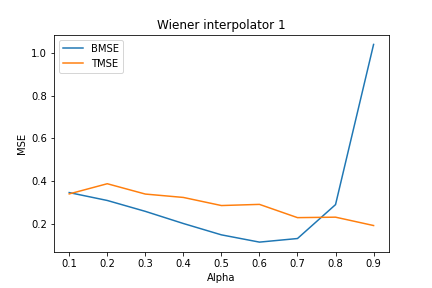
\includegraphics[width=1\linewidth]{../results/Wiener_1.png}
		\caption{MSE vs $\alpha$ for Wiener interpolator 1}
		\label{fig:wiener_1}
	\end{subfigure}%
	\begin{subfigure}{.5\textwidth}
		%\centering
		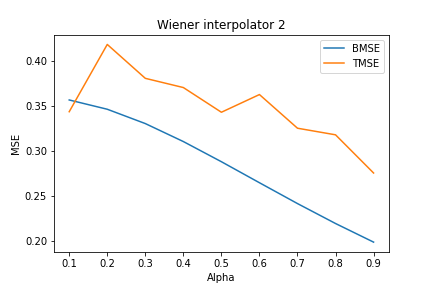
\includegraphics[width=1\linewidth]{../results/Wiener_2.png}
		\caption{MSE vs $\alpha$ for Wiener interpolator 2}
		\label{fig:wiener_2}
	\end{subfigure}
	\caption{Mean Squared Error vs $\alpha$ for Wiener interpolator}
	\label{fig:wiener}
\end{figure}


From the plot Figure(\ref{fig:wiener_1}), we can see that the Theoretical Mean Squared Error (TMSE) decreases with the increase in $\alpha$. At the same time, Bayesian Mean Squared Error (BMSE) decreases initially with $\alpha$ and after a certain value (0.6) it starts increasing. The MSE values might be high for low $\alpha$ due to numerical precision instabilities. We can also observe that the BMSE is gnerally low than TMSE for a reasonable range of $\alpha$. This interpolator seems to work better compared to its other version for low values of $\alpha$.


From the plot Figure(\ref{fig:wiener_2}), we can see that both the Theoretical Mean Squared Error (TMSE) and Bayesian Mean Squared Error (BMSE) decreases with the increase in $\alpha$. The MSE values might be high for low $\alpha$ due to numerical precision instabilities. We can also observe that the BMSE is gnerally low than TMSE for the whole range of $\alpha$. We can see that this interpolator seems to work better compared to its other version for high values of $\alpha$.



\newpage
\problem{B: Kalman filter}

\begin{figure}[h]
	\centering
	\begin{subfigure}{.5\textwidth}
		\centering
		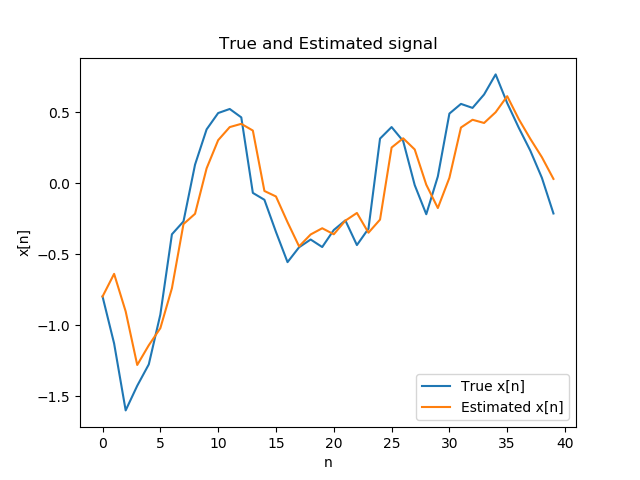
\includegraphics[width=1\linewidth]{../results/Kalman_1.png}
		\caption{True and Estimated signal}
		\label{fig:kalman_1}
	\end{subfigure}%
	\begin{subfigure}{.5\textwidth}
		\centering
		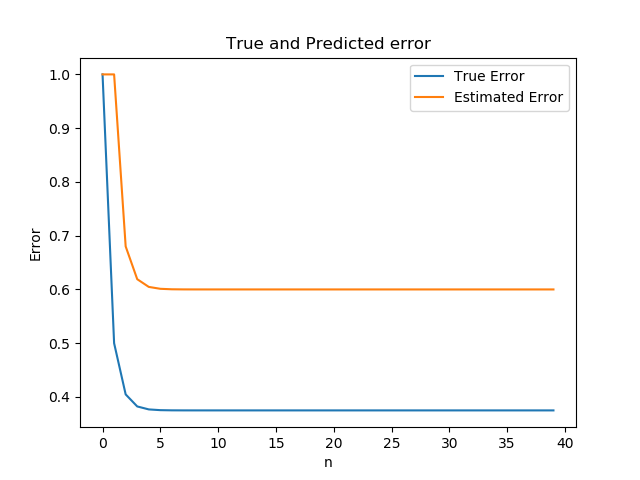
\includegraphics[width=1\linewidth]{../results/Kalman_2.png}
		\caption{True and Predicted error}
		\label{fig:kalman_2}
	\end{subfigure}
	\caption{Kalman filter}
	\label{fig:kalman}
\end{figure}


From the plot Figure(\ref{fig:kalman_1}) we can observe the true signal and estimated signal varying with $n$. Due to the random initializations, the estimated signal and true signal vary for very low values of n. But with growing n, the estimated signal tracks with true signal well. From plot Figure(\ref{fig:kalman_2}), we can observe that the true and estimated error saturate after some value for n, but the estimated error is higher compared to error.

\vspace{10em}
\problem{B: Problem 3 Comparison of causal Wiener filter and Kalman filter}

For a particular generated observation sequence $x(n)$: \\
The prediction error for Kalman filter was 0.3750. The prediction error for causal Wiener filter was 0.3600. Prediction error for Kalman filter is slightly higher than that of Wiener filter.




\newpage
\problem{C: Appendices (Python codes)}
\solution The entire program is written in six python files. The codes are provided below and are also available at \url{https://github.com/vineeths96/Interpolation-of-faulty-sensor} GitHub repository. (Repository access is private as of now. Access can me made available, if necessary).

\subproblem{wiener\_interpolator.py}
\inputminted[frame=lines, framesep=2mm, baselinestretch=1.2, fontsize=\footnotesize, linenos]{python3}{../wiener_interpolator.py}

\subproblem{kalman\_filter.py}
\inputminted[frame=lines, framesep=2mm, baselinestretch=1.2, fontsize=\footnotesize, linenos]{python3}{../kalman_filter.py}


\subproblem{wiener\_plots.py}
\inputminted[frame=lines, framesep=2mm, baselinestretch=1.2, fontsize=\footnotesize, linenos]{python3}{../wiener_plots.py}

\subproblem{kalman\_plots.py}
\inputminted[frame=lines, framesep=2mm, baselinestretch=1.2, fontsize=\footnotesize, linenos]{python3}{../kalman_plots.py}

\subproblem{comparison.py}
\inputminted[frame=lines, framesep=2mm, baselinestretch=1.2, fontsize=\footnotesize, linenos]{python3}{../comparison.py}

\subproblem{parameters.py}
\inputminted[frame=lines, framesep=2mm, baselinestretch=1.2, fontsize=\footnotesize, linenos]{python3}{../parameters.py}

\end{document} 
